\documentclass[10pt,a4paper,twocolumn]{article}
\usepackage{f1000_styles}
\usepackage{hyperref}
\usepackage{enumitem}

\begin{document}

\title{Software Carpentry: Lessons Learned}
\author[1]{Greg Wilson}
\affil[1]{Software Carpentry Foundation / gvwilson@software-carpentry.org}

\maketitle
\thispagestyle{fancy}

\begin{abstract}

Since its start in 1998, Software Carpentry has evolved from a
week-long training course at the US national laboratories into a
worldwide volunteer effort to improve researchers' computing
skills. This paper explains what we have learned along the way, the
challenges we now face, and our plans for the future.

\end{abstract}
\clearpage

\section{Introduction}

In January 2012, John Cook posted this to his widely-read blog
\cite{cook2012}:

\begin{quote}
In a review of linear programming solvers from 1987 to 2002, Bob Bixby
says that solvers benefited as much from algorithm improvements as from
Moore's law: ``Three orders of magnitude in machine speed and three
orders of magnitude in algorithmic speed add up to six orders of
magnitude in solving power. A model that might have taken a year to
solve 10 years ago can now solve in less than 30 seconds.''
\end{quote}

A million-fold speed-up is impressive, but hardware and algorithms are
only two sides of the iron triangle of programming. The third is
programming itself, and while improvements to languages, tools, and
practices have undoubtedly made software developers more productive
since 1987, the speed-up is percentages rather than orders of
magnitude.  Setting aside the minority who do high-performance
computing (HPC), the time it takes the ``desktop majority'' of
scientists to produce a new result is frequently dominated by how long
it takes to write, test, debug, install, and maintain software.

The problem is that most scientists are never taught how to do
this. Their undergraduate programs may include a generic introduction
to programming or a statistics or numerical methods course (in which
they are often expected to pick up programming on their own), but they
are almost never told that version control exists, and rarely if ever
shown how to structure a maintainable program, or how to turn the last
twenty commands they typed into a re-usable script. As a result, they
routinely spend hours doing things that could be done in minutes, or
don't do things at all because they don't know where to start
\cite{hannay2009,prabhu2011}.

This is where Software Carpentry comes in. We ran over 400 workshops
for over 12,000 researchers between January 2013 and July 2015. In
them, over 400 volunteer instructors helped attendees learn about
program design, task automation, version control, testing, and other
unglamorous but time-tested skills \cite{wilson2013}. Two independent
assessments in 2012 \cite{aranda2012,libarkin2012} and two others more
recently \cite{schossau2014,simperler2015} have indicated that this
training is helping (though as we discuss in
Section~\ref{s:assessment}, these results are still preliminary):

\begin{quote}
The program increases participants' computational understanding, as
measured by more than a two-fold (130\%) improvement in test scores
after the workshop. The program also enhances their habits and routines,
and leads them to adopt tools and techniques that are considered
standard practice in the software industry. As a result, participants
express extremely high levels of satisfaction with their involvement in
Software Carpentry (85\% learned what they hoped to learn; 95\% would
recommend the workshop to others).
\end{quote}

\section{From Red to Green}

Like many projects, it has taken us years to become an overnight
success, and we have made many mistakes along the way.  These are best
understood historically.

\subsection{Version 1: Red light}

In 1995-96, the author organized a series of articles in \emph{IEEE
Computational Science \& Engineering} titled, ``What Should Computer
Scientists Teach to Physical Scientists and Engineers?'' \cite{wilson1996}.
These grew out of the frustration he had working with scientists
who wanted to run before they could walk, i.e., to parallelize complex
programs that were not broken down into self-contained functions, that
did not have any automated tests, and that were not under version control
\cite{wilson2006a}.

In response, John Reynders (then director of the Advanced Computing
Laboratory at Los Alamos National Laboratory) invited the author and
Brent Gorda (now at Intel) to teach a week-long course to LANL staff.
This course ran for the first time in July 1998, and was repeated nine
times over the next four years. It eventually wound down as Gorda and
the author moved on to other projects, but two valuable lessons were
learned:

\begin{enumerate}

\item
  Intensive week-long courses are easy to schedule (particularly if
  instructors have to travel) but by the last two days, attendees'
  brains are full and learning drops off significantly.

\item
  Textbook software engineering is not useful to most scientists. In
  particular, careful documentation of requirements and lots of
  up-front design are not appropriate for people who (almost by
  definition) do not know what the right answer is yet. Agile
  development methods (which rose to prominence during this period)
  are a less bad fit to researchers' needs, but even they are not well
  suited to the common ``solo grad student'' model of working.

\end{enumerate}

\subsection{Versions 2 and 3: Another Red Light}

The Software Carpentry course materials were updated and released in
2004-05 under a Creative Commons license with support from the
Python Software Foundation \cite{wilson2006b}. They were used twice in
a conventional term-long graduate course at the University of Toronto
aimed at a mix of students from Computer Science and the physical and
life sciences.

The materials attracted 1000-2000 unique visitors a month.  But while
graduate students (and the occasional faculty member) found the course
at Toronto useful, it never found an institutional home.  Most
Computer Science faculty believe that this basic material is too easy
to deserve a graduate credit (even though a significant minority of
their students, particularly those coming from non-CS backgrounds,
have no better software development skills than the average
physicist). Meanwhile, other departments believe that courses like
this ought to be offered by Computer Science, in the same way that
Mathematics and Statistics departments routinely offer service
courses.  In the absence of an institutional mechanism to offer credit
courses at some inter-departmental level, this course, like many other
interdisciplinary initiatives, was left without a home.

\begin{quote}
\textbf{It works too well to be worth teaching}

Most computer scientists want to do research to advance our
understanding of the science of computing; things like command-line
history, tab completion, and ``select * from table'' have been around
too long, and work too well, to be interesting. As long as
universities reward research first, and teaching last, it is simply
not in most computer scientists' interests to offer courses like this.
\end{quote}

Secondly, despite repeated invitations, other people did not
contribute new material beyond an occasional bug report (a point which
we will return to in Section~\ref{s:lesson-collab}).

The most important lesson, though, was that while many faculty in
science, engineering, and medicine agree that their students should
learn more about computing, they \emph{won't} agree on what to take
out of the current curriculum to make room for it. A typical
undergraduate science degree in the US or Canada comprises roughly
1800 hours of class and laboratory time. Anyone who wants to add more
programming, statistics, writing, or anything else must either
lengthen the program (which is financially and institutionally
infeasible) or take something out. However, everything in the program
is there because it has a passionate defender who thinks it's vitally
important, and who is likely senior to those faculty advocating the
change.

\begin{quote}
\textbf{It adds up}

Saying, ``We'll just add a little computing to every other course,'' is
a cheat: five minutes per hour equals four entire courses in a four-year
program, which is unlikely to ever be implemented. Pushing computing
down to the high school level is also a non-starter, since that
curriculum is also full.
\end{quote}

The sweet spot for this kind of training is therefore the first years
of graduate school. At that point, students have time to learn (at
least, more time than they'll have once they're faculty) and real
problems of their own that they want to solve.

\subsection{Version 4: Orange Light}\label{s:version4}

The author rebooted Software Carpentry in May 2010 with support from
Indiana University, Michigan State University, Microsoft, MITACS,
Queen Mary University of London, Scimatic, SciNet, SHARCNet, and the
UK Met Office. More than 120 short video lessons were recorded during
the subsequent 12 months, and six week-long classes were run for the
backers. We also offered an online class three times (a MOOC
\emph{avant la lettre}).

This was our most successful version to date, in part because the
scientific landscape itself had changed. Open access publishing, crowd
sourcing, the data deluge in the life sciences, and growing concern
about reproducible research had convinced a growing number of
scientists that knowing how to program was now as important as knowing
how to do statistics.  Even most of them, though, still (rightly)
regarded it as a tax they had to pay in order to get their science
done.

Despite this round's overall success, there were several
disappointments:

\begin{enumerate}

\item
  Once again, we discovered that five eight-hour days are more wearying
  than enlightening.

\item
  And once again, only a handful of other people contributed material
  (see Section~\ref{s:lesson-collab}).

\item
  Creating videos is significantly more work than creating slides.
  Editing or modifying them is harder still: while a typo in a slide
  can be fixed by opening PowerPoint, making the change, saving, and
  re-exporting the PDF, inserting new slides into a video and updating
  the soundtrack seems to take at least half an hour regardless of how
  small the change is.  This makes maintaining a video-based course
  prohibitively expensive.

\item
  Most importantly, the MOOC format didn't work: only 5-10\% of those
  who started with us completed the course, and the majority were
  people who already knew most of the material. Both figures are in
  line with completion rates and learner demographics for other MOOCs
  \cite{jordan2013}, but that does not make them less disappointing.

\end{enumerate}

The biggest take-away from this round was the need to come up with a
scalable, sustainable model for delivering training. One instructor
simply can't reach enough people, and cobbling together funding from
half a dozen different sources every twelve to eighteen months is
risky as well as wearying.

\subsection{Version 5: Green Light}

Software Carpentry rebooted again in January 2012 with a grant from
the Sloan Foundation to the Mozilla Foundation.  This time, the model
was two-day intensive workshops like those pioneered by The Hacker
Within, a grassroots group of grad students helping grad students at
the University of Wisconsin - Madison.

Shortening the workshops made it possible for more people to attend,
and increased the proportion of the material they could absorb. It
also forced us to think much harder about what skills scientists
really needed. Out went object-oriented programming, XML, Make, and
other topics.  Instead, we focused on a small set of tools that let us
introduce higher-level concepts without learners really noticing
(Section~\ref{s:curriculum}).

Reaching more people allowed us to recruit new instructors from
workshop participants, which in turn allowed us to scale. Switching to
a ``host site covers costs'' model was equally important: funding was
still needed for 1.5 core staff to lead the project and match
instructors to workshops, but everything else funded itself.

\begin{quote}
\textbf{Learning to teach}

One of our most important discoveries during this period was that many
people are as interested in learning about better teaching practices
as they are in learning about computing.  We discuss this in detail in
Section~\ref{s:instructor-training}.

\end{quote}

\subsection{Version 6: A True Community Project}\label{s:community}

In July 2014, the author left Mozilla and set up the Software
Carpentry Foundation, an independent non-profit foundation under the
auspices of NumFOCUS.  The SCF held its first elections in January
2015, in which instructors who had taught over the past two years
selected seven of their own number as a Steering Committee to oversee
the project's operations.  Since then, the SCF has formed partnerships
with a growing number of institutions (see
Table~\ref{t:current-partners}), run an ever-increasing number of
workshops, and much more.

While the SCF is only nine months old, we have already learned many
things.  The most important are:

\begin{enumerate}

\item
  The first few people to join a volunteer organization are usually
  keener than those who join later.  As numbers grow, therefore, the
  time contributed per person will decrease, and structures must be
  designed with this in mind.  In particular, by the time there 400
  people are on the books, most will be dipping in and out of
  conversations rather than taking part on a daily or weekly basis, so
  frameworks and procedures must become simple and stable.

\item
  Every partner organization has different needs and
  constraints\footnote{We have learned much more than we ever wanted
    to about accounting rules at various universities\ldots}.
  ``Standard'' partnership agreements therefore have to
  be treated as starting points for negotiation, rather than as ``take
  it or leave it'' propositions.

\item
  ``Bikeshedding'' is the practice of arguing over minor, marginal
  issues while more serious ones are overlooked.  It is a constant
  danger in an organization whose more vocal members actually enjoy
  programming.  Squelching such technical discussions has a chilling
  effect on conversation overall, but letting them go unchecked
  alienates people who would rather talk about teaching, or simply
  don't have enough time to go down technical rabbit holes.  We
  discuss an example in Sections~\ref{s:lesson-templates}
  and~\ref{s:editors}.

\end{enumerate}

\subsection{Data Carpentry}

The biggest recent development, though, has been the foundation of a
sibling organization called Data Carpentry in April 2014.  Where
Software Carpentry's mission is to help scientists who are programming
badly to program better, Data Carpentry's focus is, as its name
implies, to help them manage and analyze their data.  Led by
Dr.\ Tracy Teal, Data Carpentry was recently awarded \$700,000 by the
Moore Foundation, and is expected to grow rapidly over the coming two
years.

\subsection{Results}

As we discuss in Section~\ref{s:assessment}, we do not know how to
measure the impact of our workshops.  However, both their number, and
the number of people attending, have grown steadily:

\begin{figure}
\centering
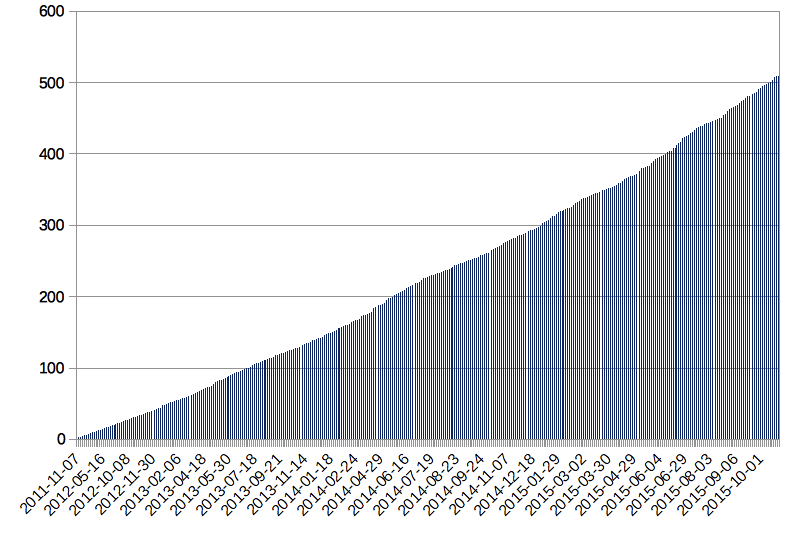
\includegraphics[width=0.4\textwidth]{workshops.png}
\caption{Cumulative Number of Workshops}
\label{f:workshops}
\end{figure}

\begin{figure}
\centering
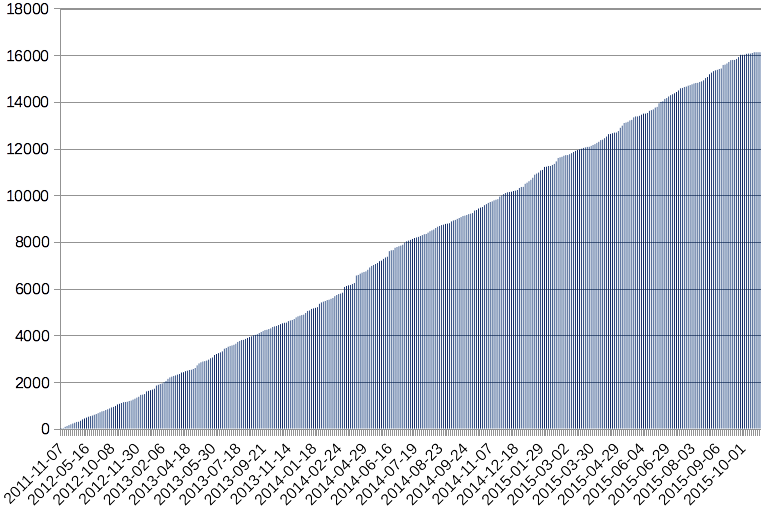
\includegraphics[width=0.4\textwidth]{learners.png}
\caption{Cumulative Number of Learners}
\label{f:enrolment}
\end{figure}

\begin{figure}
\centering
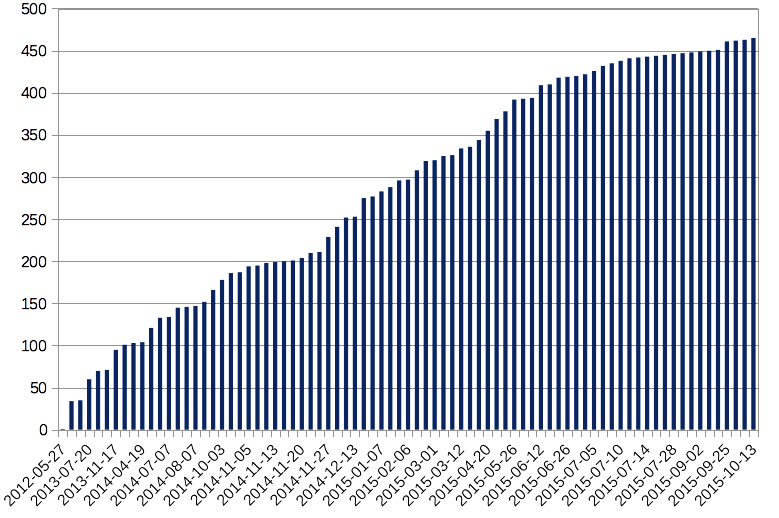
\includegraphics[width=0.4\textwidth]{instructors.png}
\caption{Cumulative Number of Instructors}
\label{f:instructors}
\end{figure}

We are now a truly global organization (Table~\ref{t:by-country}).
And most importantly, feedback from participants is strongly positive.
While there are always problems with software set-up and the speed of
instruction (Section~\ref{s:instruction-pace}), 80-90\% of attendees
typically report that they were glad they attended and would recommend
the workshops to colleagues.

\section{What we do}\label{s:curriculum}

So what does a typical workshop look like?

\begin{itemize}
\item
  \emph{Day 1 a.m.}: The Unix shell. We only show participants a dozen
  basic commands; the real aim is to introduce them to the idea of
  combining single-purpose tools (via pipes and filters) to achieve
  desired effects, and to getting the computer to repeat things (via
  command completion, history, and loops) so that people don't have
  to.
\item
  \emph{Day 1 p.m.}: Programming in Python, R, or MATLAB. (Only one
  language is taught in any given workshop.) The real goal is to show
  them when, why, and how to grow programs step-by-step as a set of
  comprehensible, reusable, and testable functions.
\item
  \emph{Day 2 a.m.}: Version control. We begin by emphasizing how this
  is a better way to back up files than creating directories with names
  like ``final'', ``really\_final'', ``really\_final\_revised'', and
  so on, then show them that it's also a better way to collaborate
  than FTP or Dropbox.
\item
  \emph{Day 2 p.m.}: Either more about programming in the workshop's
  chosen language, or an introduction to databases and SQL.  If the
  latter is chosen, the real goal is to show them what structured data
  actually is (in particular, why atomic values and keys are
  important) so that they will understand why it's important to store
  information this way.
\end{itemize}

As the descriptions above suggest, our real aim isn't to teach any
specific tool: it's to teach \emph{computational competence}. We can't
do this in the abstract: people won't show up for a hand-waving talk
about general principles because they won't believe those principles
will help them meet next Thursday's deadline.  Even if they do, they
won't understand, because big ideas need to be grounded in specific
examples to be comprehensible. If we show them how to solve a specific
problem with a specific tool, we can then lead into a larger
discussion of how scientists ought to develop, use, and curate
software.

There are a lot of local variations around the curriculum shown above.
For example, some instructors use the command-line Python interpreter,
while others prefer the \href{https://jupyter.org/}{Jupyter Notebook}.
Still others teach R or MATLAB instead, while a handful of workshops
also cover tools such as LaTeX, or domain-specific topics such as
audio file processing, depending on the needs of the audience and the
expertise of the instructor.

We aim for no more than 40 people per room at a workshop, so that
every learner can receive personal attention when needed.  Where
possible, we run two or more rooms side by side, and use a
pre-assessment questionnaire to stream learners by prior experience,
which simplifies teaching and improves their experience.  We do
\emph{not} shuffle people from one room to another between the first
and second day: with the best inter-instructor coordination in the
world, doing so would result in lost context.

Our workshops are sometimes free, but most now charge a small
registration fee (typically \$20-40), primarily because it reduces the
no-show rate from a third to roughly 5\%.  When this is done, we must
be careful not to trip over institutional rules about commercial use
of their space: some universities will charge hundreds or thousands of
dollars per day for use of their classrooms if any money changes
hands.  As this is usually several times more than a small
registration fee would bring in, we usually choose the higher no-show
rate as the lesser evil\footnote{We have also experimented with
  refundable deposits, but the administrative overheads were
  unsustainable.  It also does not help get around the rules mentioned
  in the previous paragraph, since money still appears to be changing
  hands in the university's eyes.}.

\begin{quote}
\textbf{Commercial offerings}

Our material \cite{swcsite,swcgithub} is all covered by the Creative
Commons Attribution license, so anyone who wants to use it for
commercial training can do so without explicit permission from us. We
encourage this: if graduate students can help pay their bills by
sharing what they know, in the way that many programmers earn their
living by working on open source software, our community will only be
stronger.

What \emph{does} require permission is use of our name and logo, both
of which are trademarked.  Such permission is granted automatically if
at least one instructor is certified, the workshop covers three core
topics (the shell, version control, and a programming langauge), and
the organizers send us summary information (the dates, the location,
and the number of attendees).  We put these rules in place because of
people calling something ``Software Carpentry'' when they had nothing
to do with what we usually teach. We have worked hard to create
material that actually helps scientists, and to build some name
recognition around it, and we would like to make sure our name
continues to mean something.
\end{quote}

\begin{quote}
\textbf{Administration fees}

If the Software Carpentry Foundation helps to organize a workshop
(e.g., finds instructors and handles registration) then we charge the
host site a \$2500 administration fee.  This fee, which currently
provides about a quarter of our revenue, is routinely waived for
workshops in under-served areas and developing countries.  If host
sites organize the workshop themselves, we will still set up
registration and send out pre- and post-workshop questionnaires.
There is no fee in this case, but we do ask for a donation (we suggest
\$500).

\end{quote}

As well as instructors, we rely on local helpers to wander the room
and answer questions during practical sessions. These helpers may be
alumni of previous workshops who are interested in becoming
instructors, grad students who have picked up some or all of our core
skills on their own, or members of the local open source community;
where possible, we aim to have at least one helper for every eight
learners.

We find workshops go a lot better if people come in groups (e.g., 4-5
people from one lab) or have other pre-existing ties (e.g., are
working in the same field). They are less inhibited about asking
questions, and can support each other (morally and technically) when
the time comes to put what they've learned into practice after the
workshop is over. Group sign-ups also yield much higher turnout from
groups that are otherwise often under-represented, such as women and
minority students, since they know in advance that they will be in a
supportive environment.

\section{Small things add up}

As in chess, success in teaching often comes from the accumulation of
seemingly small advantages. Here are a few of the things we do that we
believe have contributed to our success.

\subsection{Feedback loops}\label{s:feedback}

Giving each learner two sticky notes of different colors allows
instructors to do quick true/false questions as they're teaching. It
also allows real-time feedback during hands-on work: learners can put
a green sticky note on their laptop when they have something
completed, or a red one when they need help.

We also use them as minute cards: before each break, learners take a
minute to write one thing they've learned on the green sticky note,
and one thing they found confusing (or too fast or too slow) on the
red. It only takes a couple of minutes to collate these, and allows
the instructors to adjust to learners' interests and speed.

We frequently also ask for summary feedback at the end of each day.
The instructors ask the learners to alternately give one positive and
one negative point about the day, without repeating anything that has
already been said.  This requirement forces people to say things they
otherwise might not: once all the ``safe'' feedback has been given,
participants will start saying what they \emph{really} think.

\begin{quote}
\textbf{Different channels, different messages}

Minute cards are anonymous; the alternating up-and-down feedback is
not.  Each mode has its strengths and weaknesses, and by providing
both, we hope to get the best of both worls.
\end{quote}

On a longer timescale, we send a post-workshop assessment
questionnaire to attendees shortly after the workshop ends.  Response
rates vary, but are usually low, and the opt-in nature of the survey
undoubtedly biases the data (Section~\ref{s:assessment}).  Feedback
from instructors has proven more insightful.  In August 2015, for
example, Azalee Bostroem surveyed our instructors to find out what
they were actually teaching about
Python\footnote{http://software-carpentry.org/blog/2015/09/thinking-about-teaching.html.}
From this, we learned that 60\% of our learners are novices with
little or no prior programming experience, and that only a third of
workshops get through the entire Python lesson.

Finally, starting in January 2015 we began running biweekly debriefing
sessions for instructors who have recently taught workshops, in which
they can discuss what they actually did, how it worked, how the
lessons they actually delivered differed from our templates, what
problems arose, and so on.  Summaries are posted shortly after each
meeting, and Alistair Walsh recently collected and posted information
about the same Python lesson discussed
above\footnote{http://software-carpentry.org/blog/2015/10/python-debriefing-summary.html}.
We are now (October 2015) beginning a redesign of the lesson to take
all this information into account.

\subsection{Live coding}

We teach via live coding rather than using slides because:

\begin{itemize}

\item Watching code emerge on the screen is much more convincing than
  looking at pre-made slides.

\item It enables instructors to be more responsive to ``what if?''
  questions.

\item It facilitates lateral knowledge transfer (e.g., people learn
  about keyboard shortcuts and efficient search/replace strategies in
  the editor as well as Python).

\item It slows instructors down: if they have to type in code as they
  go along, they can only go twice as fast as their learners instead
  of ten times as fast.  (And once instructors get in the habit of
  saying everything twice---once as they're typing, and a second time
  to recapitulate, pointing at the screen---most learners are able to
  keep up.)

\item Learners get to see instructors's mistakes \emph{and how they
  diagnose and fix them}.  Learners frequently report that this is the
  most valuable part of the workshop: as novices, they're going to
  spend most of their time trying to figure out what's gone wrong and
  how to fix it, so it's very valuable to see which parts of error
  messages instructors pay attention to, and what steps they take to
  correct mistakes.

\end{itemize}

It takes a bit of practice for instructors to
get used to thinking aloud while coding in front of an audience, but
most report that it is then no more difficult to do than talking off a
deck of slides.

\begin{quote}
\textbf{One device good, two devices better}

Many instructors now use two devices when teaching: a laptop plugged
into the projector for learners to see, and a tablet beside it on
which they can view their notes and the Etherpad session
(Section~\ref{s:etherpad}).  This seems to be more reliable than
displaying one virtual desktop while flipping back and forth to
another.
\end{quote}

\subsection{Open everything}

Our grant proposals, mailing lists, and everything else that isn't
personally sensitive are out in the open (see \cite{swcsite} for
links).  We believe that letting people see us succeed, fail, and
learn encourages them to be more involved in our community, and
inspires them to be open as well.

\subsection{Open lessons}

This is an important special case of the previous point. Anyone who
wants to use our lessons can take what we have, make changes, and
offer those back by sending us a pull request on GitHub. As discussed
in Section~\ref{s:lesson-collab}, this workflow is foreign to most
educators, but allows us to scale and adapt more quickly and more
cheaply than the centralized approaches being taken by many
high-profile online education ventures.

For example, we recently ``published'' our core lessons through
\href{https://zenodo.org/}{Zenodo}.  The number of contributors per
lesson is shown in Table~\ref{t:authors-per-lesson}.  The distribution
of contributions has the usual long-tail distribution, but the fact
remains that our lessons have had more contributors than many
``massive'' and ``open'' online courses.

\subsection{Use what we teach}

We also make a point of eating our own cooking, e.g., we use GitHub
for our web site and to plan workshops. Again, this makes us more
credible, and gives instructors hands-on practice with the things
they're going to teach.  Up until a year ago, the (considerable)
downside to this was that it could be difficult for newcomers to
contribute material.  We have simplified our templates and build
procedures considerably to fix this, and will be making more changes
early in 2016 to incorporate further insights.

One problem we haven't solved is the bikeshedding mentioned earlier.
Many contributors would rather spend days tweaking the build process
for lessons rather than an hour coming up with some new self-test
exercises for those same lessons, both because they are on more
familiar ground when debating programming issues, and because the
feedback loop is much tighter.  One of our goals for the coming year
is to push the bulk of discussion toward teaching practices and lesson
content.

\subsection{Meet the learners on their own ground}

Learners tell us that it is important to them to leave the workshop
with their own machine set up to do real work.  We therefore continue
to teach on all three major platforms (Linux, Mac OS X, and Windows),
even though it would be simpler to require learners to use just one
(Section~\ref{s:installation}).

We have experimented with virtual machines (VMs) on learners'
computers to reduce installation problems, but those introduce
problems of their own: older or smaller machines simply aren't fast
enough, and learners often struggle to switch back and forth between
two different sets of keyboard shortcuts for things like copying and
pasting.

Some instructors use VPS over SSH or web browser pages instead.  This
solve the installation issues, but makes us dependent on host
institutions' WiFi (which can be of highly variable quality), and
has the issues mentioned above with things like keyboard shortcuts.

\subsection{Collaborative note-taking}\label{s:etherpad}

We often use \href{http://etherpad.org}{Etherpad} for collaborative
note-taking and to share snippets of code and small data files with
learners. (If nothing else, it saves us from having to ask students to
copy long URLs from the presenter's screen to their computers.) It is
almost always mentioned positively in post-workshop feedback, and
several workshop participants have started using it in their own
teaching.

\subsection{Pair programming}

Pairing is a good practice in real life, and an even better way to
teach: partners can not only help each other out during the practical,
but can also clarify each other's misconceptions when the solution is
presented, and discuss common research interests during breaks. To
facilitate this, we strongly prefer flat (dinner-style) seating to
banked (theater-style) seating; this also makes it easier for helpers
to reach learners who need assistance.

\subsection{Diversity}

On June 24-25, 2013, we ran our first workshop for women in science,
engineering, and medicine. This event attracted 120 learners, 9
instructors, a dozen helpers, and direct sponsorship from several
companies, universities, and non-profit organizations. Our second such
workshop ran in March 2014, and we have done half a dozen of varying
sizes since.  While we do occasionally get complaints (mostly from
outsiders) about such events being discriminatory, they are
overwhelmed by the uniformly positive response from participants, many
of whom say that they would probably not have attended a mixed-gender
event because of previous bad experiences with tech meetups.

\section{Instructor training}\label{s:instructor-training}

The instructor training program that we started in August 2012 has
attracted hundreds of participants, and at the time of writing there
are over 400 more on the waiting list.  This introduction to modern
research in education and evidence-based teaching practices
\cite{hlw2010} doesn't just improve our teaching: it also helps give
the instructors a sense of community and purpose.

In its original form, training took 2-4 hours/week of participants'
time for 12-14 weeks (depending on scheduling interruptions); more
recently, we have run it both as a live two-day event, and as a
two-day online event, in which participants are together in groups of
half a dozen or more at one, two, or three sites, while the instructor
takes part over the web.

This training course introduces participants to the basics of
educational psychology, instructional design, and how these things
apply to teaching programming
\cite{guzdial2010,guzdial2013,hazzan2011,porter2013,sorva2012}. It is
necessarily very shallow, but most participants find the material
interesting as well as useful.  Introducing grad students and faculty
to evidence-based teaching practices may turn out to be Software
Carpentry's greatest contribution.

\subsection{Why teach?}

But why do people volunteer as instructors?

\begin{itemize}

\item \emph{To make the world a better place.}  The two things we
  need to get through the next hundred years are more science and more
  courage; by helping scientists do more in less time, we are helping
  with the former.

\item \emph{To make their own lives better.}  Our instructors are
  often asked by their colleagues to help with computing problems.
  The more those colleagues know, the more interesting those requests
  are.

\item \emph{To network.}  Showing up to run a workshop is a great way
  for people to introduce themselves to colleagues and make contact
  with potential collaborators. This is probably the most important
  reason from Software Carpentry's point of view, since it's what
  makes our model sustainable.

\item \emph{To practice teaching.}  This is also important to people
  contemplating academic careers.
 
\item \emph{To help diversify the pipeline.}  Computing is 12-15\%
  female, and that figure has been \emph{dropping} since its high
  point in the 1980s \cite{wic}. Some of our instructors are
  involved in part because they want to help break that cycle by
  participating in activities like our workshops for women in science
  and engineering.

\item \emph{To learn new things, or learn old things in more detail.}
  Working alongside an instructor with more experience is a great way
  to learn more about the tools, as well as about teaching.

\item \emph{It's fun.}  Our instructors get to work with smart people
  who actually want to be in the room, and don't have to mark anything
  afterwards. It's a refreshing change from teaching undergraduate
  calculus\ldots{}

\end{itemize}

\section{Collaborative Lesson Development}\label{s:lesson-collab}

Large-scale ad hoc collaboration is the norm in open source software
development and the creation of encyclopedia articles, but is still
rare in other fields. In particular, teachers often use one another's
slide decks as starting points for their own courses, but rarely offer
their changes back to the original author in order to improve
them. This is only partly because educators' preferred file formats
(Word, PowerPoint, and PDF) aren't handled gracefully by existing
version control systems.  A deeper cause is that there isn't a culture
of contribution, particularly in higher education.

The question is, why not?  Reasons advanced include:

\begin{itemize}

\item \emph{Lack of technical skill.} But (a) many teachers edit
  Wikipedia, and (b) a large number of those who teach programming
  certainly \emph{do} have the technical skills.

\item \emph{Lack of institutional rewards.} But if this was a real
  barrier, open source software and Wikipedia wouldn't exist.

\item \emph{Episodic interaction.} If someone is teaching a full or
  half-year course, they may only revisit the material every six
  months to a year, and the context in which it's taught may well be
  different.

\item \emph{It just hasn't happened yet.} This argument might have
  been tenable a decade ago, but is less credible with every passing
  year.

\end{itemize}

Our current hypothesis is that teaching is \emph{enacted knowledge}
\cite{fincher2007,fincher2012}.
To make a musical analogy, the lesson plan, slides, and assignments
are only the score; what matters most is how it's performed.  If this
is correct, then collaborative lesson development will only succeed if
it is done as part of what the Japanese call \emph{jugyokenkyu}
(lesson study): the systematic observation and discussion of lessons
by fellow teachers.

In aid of this, in January 2015 we began running bi-weekly debriefing
sessions for instructors who have recently taught workshops (see
Section~\ref{s:feedback}).  We are also planning to revise instructor
training to require trainees to watch and reflect on videos of
experienced instructors delivering our lessons.  We hope that making
this ``the new normal'' will encourage even more collaboration on the
content and delivery of our lessons.

\section{Example: lesson templates}\label{s:lesson-templates}

Section~\ref{s:community} mentioned that we have spent more time
wrangling over technical details (``bikeshedding'') than we should
have, at the expense of discussing pedagogy and lesson content.  The
prime example of this is probably the way we format our lessons: we
have invested hundreds of hours in debating and implementing various
options.  Over the years, we have tried the following:

\begin{itemize}

\item \emph{HTML.}  People (rightly) complained about editing HTML
  tags was annoying, and about maintaining forward/backward links and
  glossary entries by hand.

\item \emph{XML with a custom translation tool.}  This had all the
  disadvantages of HTML, with extra overhead of maintaining the
  XML-to-HTML translation tool.

\item \emph{A wiki.} The tool used didn't handle concurrent edits
  gracefully, and didn't provide any mechanism for pre-publication
  review.  We could live without the former if the latter worked, but
  the wiki tools available at the time also didn't provide a way to
  indicate the semantics of specific regions, e.g., to signal that
  this part of the lesson was the objectives, while that was an
  exercise.

\item \emph{All lessons in one big repository.}  This was
  unsatisfactory for (at least) three reasons:

  \begin{enumerate}

  \item Putting everything in one repository made that repository
    uncomfortably large to clone.

  \item If people subscribed to notifications for the repository, they
    were inundated with notices about changes to lessons they didn't
    care about.

  \end{enumerate}

  At the same time, we experimented with using \href{Jupyter
  Notebooks}{http://jupyter.org/} to author lessons.  Notebooks are
  a wonderful tool for doing real scientific work, but less well
  suited to large-scale collaboration.  In particular, while it's
  possible for experienced users to diff and merge Jupyter Notebooks,
  it is intimidating and error-prone for newcomers (particularly in
  the face of embedded images).\footnote{The irony of telling people
    not to use ``binary'' formats like Microsoft Word for documents
    because they don't play nicely with version control, and then
    using a format that is almost as awkward, did not escape our
    users{\ldots}}


\item \emph{Markdown and HTML in a single GitHub repository per lesson
  with a custom build.}
  Markdown files in the \texttt{gh-pages} branch of a GitHub repository
  will be automatically translated into HTML using a tool called
  Jekyll, and those HTML pages will then be published as a website.
  This is great---except that Jekyll can't translate Jupyter
  Notebooks or R Markdown files, so we have to pre-process those and
  commit the results to the repository.  We decided that if we're
  doing that, we might as well go the whole way, i.e., generate the
  HTML ourselves and commit that to the \texttt{gh-pages} branch rather
  than run Jekyll on the server at all.

  Another problem is that many things can only be expressed in
  Markdown by using HTML directly.  In particular, there is no way to
  create \texttt{div} elements to represent things like callout boxes,
  exercises, lesson goals, and so on.  We have resorted to using
  blockquotes for all of these, with some post-processing and CSS
  tricks to get the appearance we want.

\end{itemize}

Our next step (which we plan to implement in December 2015) is to take
advantage of some of the extra features of one of the dialects of
Markdown that Jekyll supports to solve the styling problem, so that we
can store only the Markdown files in the GitHub repository, rather
than the generated HTML.  This will simplify things for newcomers, but
we will still need custom build steps to handle Jupyter Notebooks, R
Markdown, and other file formats, and the intermediate files produced
by those build steps will still need to be kept in the repository.

Stepping back, what we have learned from wrangling formats is:

\begin{enumerate}

\item \emph{There are no good answers.}  Every currently-available
  option for publishing moderately complex material (such as lessons
  and scientific papers) is broken in some way.

\item \emph{Fixing things is often a mistake.}  Or rather, fixing
  things \emph{frequently} is: as one of our instructors pointed out
  in the summer of 2015, every time he had taught a workshop in the
  previous three years, the process for setting up, formatting
  lessons, and so on had changed.  We are now committed to updating
  our templates and processes no more than once a year.

\item \emph{The best templates and platforms in the world won't make
    writing lessons easy.}  The best we can hope to achieve is to
  make it less hard.

\end{enumerate}

\section{TODO}

We've learned a lot, and we're doing a much better job of reaching and
teaching people than we did three years ago, but there are still many
things we need to improve.

\subsection{Long-term assessment}\label{s:assessment}

Our biggest challenge is figuring out whether we are actually helping
scientists get more science done, and if so, how, and how much.
\cite{aranda2012,libarkin2012,schossau2014,simperler2015} seem to show
that we are, but we have not yet done a large-scale, long-term
follow-up. This is partly because of a lack of resources, but it is
also a genuinely hard problem: no one knows how to measure the
productivity of programmers, or the productivity of scientists, and
putting the two together doesn't make the unknowns cancel out.

\begin{quote}
\textbf{Meeting our own standards}

One of the reasons we need to do long-term follow-up is to find out
for our own benefit whether we're teaching the right things the right
way.  As just one example, some of us believe that Subversion is
significantly easier for novices to understand than Git because there
are fewer places data can reside and fewer steps in its normal
workflow. Others believe just as strongly that there is no difference,
or that Git is actually easier to learn. While the large social
network centered around GitHub is a factor in our choice as well, we
would obviously be able to make better decisions if we had more
quantitative data to base them on.
\end{quote}

\subsection{Too slow \emph{and} too fast}\label{s:instruction-pace}

Our second biggest challenge is the diversity of our learners'
backgrounds and skill levels. No matter what we teach, and how fast or
how slow we go, 20\% or more of the room will be lost, and there's a
good chance that a different 20\% will be bored.

The obvious solution is to split people by level, but if we ask them
how much they know about particular things, they regularly under- or
over-estimate their knowledge.  We have therefore developed a short
pre-assessment questionnaire that asks them how easily they could do a
small number of specific tasks.  It is useful, in that it gives
instructors some idea of who they're going to be helping, but we have
done nothing to validate the questions themselves, i.e., to ensure
that respondents are interpreting them the same way that we are, or
that their categorization of respondents corresponds in any meaningful
way to actual proficiency.  As mentioned in Section~\ref{s:assessment},
we have been trying for several years to find the support needed to do
rigorous assessment of this and other aspects of our program, but if
funders are reluctant to invest in training, they are doubly reluctant
to invest in measuring its effects.

\subsection{``Is it supposed to hurt this much?''}\label{s:installation}

Third, getting software installed is often harder than using it. This
is a hard enough problem for experienced users, but almost by
definition our audience is \emph{inexperienced}, and our learners
don't (yet) know about system paths, environment variables, the
half-dozen places configuration files can lurk on a modern system, and
so on. Combine that with two versions of Mac OS X, three of Windows,
and two oddball Linux distributions, and it's almost inevitable that
every time we introduce a new tool, it won't work as expected (or at
all) for at least one person in the room. Detailed documentation has
not proven effective: some learners won't read it (despite repeated
prompting), and no matter how detailed it is, it will be
incomprehensible to some, and lacking for others.

\subsection{Editors}\label{s:editors}

Editing text should be a minor problem, but if you're standing in
class telling three sets of users, "Now open Notepad++ if you're on
Windows, or Kate if you're on Linux, or TextMate if you're on a Mac,
or whatever you want to use if you're more advanced", and then
demonstrate with whichever you have on your laptop (which looks
different from what half of your learners are sitting in front of),
you wll cause mass confusion.

We therefore still use \href{Nano}{http://www.nano-editor.org/} as an
editor in class, even though none of our instructors use it for real
work.  Arguments over this are another example of the bikeshedding
discussed in Section~\ref{s:lesson-templates}: many people who are
passionate about programming are also passionate (some might say
``zealous'') about their favorite editor, and will argue about the
relative merits of various choices at length.

The choice of editor is also an example of \emph{expert blind spot}.
People who know a subject well often have trouble re-imagining it
through novice eyes, and hence under-estimate how difficult ``simple''
tasks actually are for newcomers.  For example, every reasonably
experienced user of the shell knows that an editor can run inside a
terminal window, so that a single fixture on the screen can play
multiple roles.  This is \emph{not} obvious to newcomers, who are
frequently confused when instructors move back and forth between an
editor and a regular shell prompt in a single window.

\subsection{Testing}

We no longer include software testing in our core curriculum, despite
believing that it's extremely important.  The reason is that while the
mechanics of unit testing with an xUnit-style framework are
straightforward, and it's easy to come up with representative test
cases for things like reformatting data files, we don't know what to
teach scientists about testing their particular applications.  Once
we've covered floating-point roundoff and the need to use ``almost
equal'' instead of ``exactly equal'', our learners quite reasonably
ask, ``What should I use as a tolerance for my computation?'' for
which nobody has a good answer.  An attempt in 2014--15 to collect
shareable examples was unfruitful, but we hope to take another run at
this in 2016.

\subsection{Watching vs.\ doing}

We try to make our teaching as interactive as possible, but we still
don't give learners hands-on exercises as frequently as we should.  We
also don't give them as diverse a range of exercises as we should.
This is simply due to a lack of time: two eight-hour days are as much
as learners' brains can handle, but not nearly enough to give them all
the practice they need.

There is also a constant tension between having students do realistic
exercises drawn from actual scientific workflows, and giving them tasks
that are small and decoupled, so that failures are less likely and don't
have knock-on effects when they occur. This is exacerbated by the
diversity of learners in the typical workshop.

\subsection{Less of a Problem}

One issue which is less of a problem than it used to be is financial
sustainability. The ``host site covers costs'' model scales naturally
with the number of workshops, while a growing number of organizations
are keen to partner with us, primarily to build local capacity to run
more workshops when and as needed.  While we do not wish to tempt
fate, the Software Carpentry Foundation does seem to be headed toward
financial stability.

\section{Conclusions}

To paraphrase William Gibson, the future is already here: it's just
that the skills needed to implement it aren't evenly distributed. A
small number of scientists can easily build an application that scours
the web for recently-published data, launch a cloud computing node to
compare it to home-grown data sets, and push the result to a GitHub
account; others are still struggling to free their data from Excel and
figure out which of the nine backup versions of their paper is the one
they sent for publication.

The fact is, it's hard for scientists to do the cool things their
colleagues are excited about without basic computing skills, and
impossible for them to know what other new things are possible. Our
ambition is to change that: not just to make scientists more productive
today, but to allow them to be part of the changes that are transforming
science in front of our eyes. If you would like to help, we'd like to
hear from you: please mail us at admin@software-carpentry.org.

\subsection{Competing Interests}

The author is an employee of the Software Carpentry Foundation. Over
the years, Software Carpentry has received support from the
organizations listed in Section~\ref{s:version4} and
Table~\ref{t:current-partners}, and from The Mathworks, Enthought
Inc., Continuum Analytics, the Sloan Foundation, and the Mozilla
Foundation.

\subsection{Grant Information}

Software Carpentry is not currently supported by grants.

\subsection{Acknowledgements}

The author wishes to thank Brent Gorda, who helped create Software
Carpentry sixteen years ago; the hundreds of people who have helped
organize and teach workshops over the years; and the thousands of
people who have taken a few days to learn how to get more science
done in less time, with less pain.

\section{Tables}

\begin{table}[h]
\begin{tabular}{l}
Berkeley Institute for Data Science \\
Compute Canada \\
GitHub \\
Insight Data Science \\
iPlant \\
Lawrence Berkeley National Laboratory \\
Michigan State University \\
Netherlands eScience Center \\
New Zealand eScience Infrastructure \\
Oklahoma State University \\
RStudio \\
Software Sustainability Institute \\
University College London \\
UCAR \\
University of California Davis \\
University of Colorado \\
University of Florida \\
University of Leeds \\
University of Melbourne \\
University of Michigan \\
University of Oklahoma \\
University of Washington \\
\end{tabular}
\caption{Current Partners (November 2015)}
\label{t:current-partners}
\end{table}

\begin{table}[h]
\begin{tabular}{ll}
\textbf{Topic} & \textbf{Contributors} \\
Git & 55 \\
Mercurial & 25 \\
MATLAB & 28 \\
Python & 52 \\
R & 49 \\
Unix Shell & 64 \\
SQL & 41
\end{tabular}
\caption{Authors per Lesson}
\label{t:authors-per-lesson}
\end{table}

\begin{table}[h]
\begin{tabular}{lrr}
\textbf{Country} & \textbf{Workshops} & \textbf{Instructors} \\
United States & 216 & 232 \\
Canada & 59 & 52 \\
United Kingdom & 43 & 50 \\
Australia & 33 & 41 \\
Brazil & 9 & 2 \\
South Africa & 6 & 1 \\
New Zealand & 5 & 8 \\
Norway & 5 & 3 \\
Germany & 5 & 9 \\
South Korea & 4 & 1 \\
France & 3 & 3 \\
Poland & 3 & 5 \\
Switzerland & 3 & 0 \\
Italy & 2 & 1 \\
Netherlands & 2 & 0 \\
Spain & 2 & 3 \\
China & 1 & 1 \\
Cyprus & 1 & 0 \\
Denmark & 1 & 2 \\
Finland & 1 & 0 \\
Ghana & 1 & 0 \\
Indonesia & 1 & 0 \\
Jordan & 1 & 0 \\
Lebanon & 1 & 0 \\
Saudi Arabia & 1 & 0 \\
Sweden & 1 & 2 \\
Thailand & 1 & 2 \\
India & 0 & 1 \\
\end{tabular}
\caption{Workshops and Instructors by Country (October 2015)}
\label{t:by-country}
\end{table}

\clearpage

\nocite{*}
{\small\bibliographystyle{unsrt}
\bibliography{software-carpentry-lessons-learned}}

\end{document}
